\documentclass[11pt]{article}

\usepackage[margin=1in]{geometry}
\usepackage{listings}
\usepackage{graphicx}
\usepackage{subfigure}
\usepackage{subcaption} % For subfigures
\usepackage{float} % for H option in figures
\usepackage{url}
\usepackage{float}
\usepackage{amsmath}
\usepackage{amsfonts}
\usepackage{hyperref}
\usepackage{wrapfig}
\usepackage[htt]{hyphenat}
\usepackage{mathrsfs} % https://www.ctan.org/pkg/mathrsfs
    
\usepackage{biblatex} %Imports biblatex package
\addbibresource{../../../source/bibliography.bib} %Import the bibliography file

\setlength{\parindent}{0pt}

\title{Universal Segmentator}
\author{Anton Zhitomirsky}

\begin{document}

\maketitle

\href{https://universeg.csail.mit.edu/}{Home page} and paper at \cite{universeg}.

\section{Aim}

The developers are aware of a problem that deep learning models are not able to generalize to unseen segmentation tasks involving new anatomies. They are aware that developing new models will require resourcse and expertise to train their models. Specifically, they criticise the approach of transfer learning in the mdeical domain because of the differences in data size, features and task specifications between domains, and importantly still requires substaintial retrianing. 

\vspace{1em}

Therefore, UniSeg is a model that can solve unseen medical segmentation tasks without additional training. It uses a Cross-Block mechanism (Section \ref{sec:cross-block}). See the architectural approach at Figure \ref{fig:arch-comparison}.

\section{Method}

\begin{figure}[H]
    \centering
    \subfigure[Comparison between traditional architectures and proposed architecture for UniverSeg]{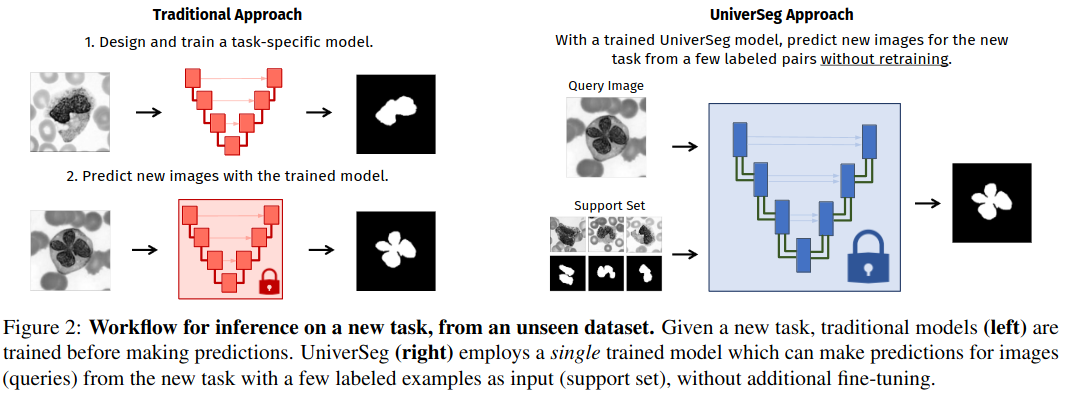
\includegraphics[width=\linewidth]{images/universeg-comparison.png}}
    \subfigure[Zoomed in view of the UniverSeg architecture]{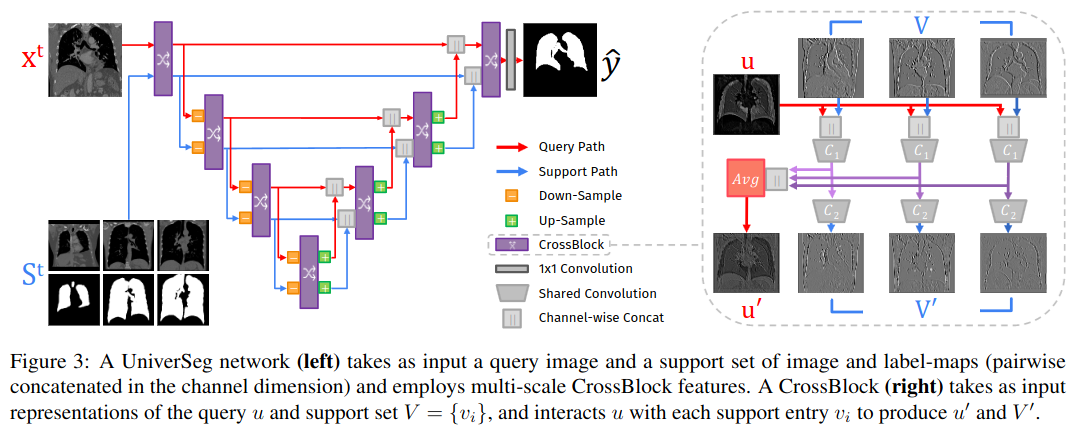
\includegraphics[width=\linewidth]{images/universeg-arch.png}}
    \caption{Taken from \cite{universeg}}\label{fig:arch-comparison}
\end{figure}



\section{Cross Block} \label{sec:cross-block}

\printbibliography

\end{document}